\PassOptionsToPackage{unicode=true}{hyperref} % options for packages loaded elsewhere
\PassOptionsToPackage{hyphens}{url}
%
\documentclass[]{article}
\usepackage{lmodern}
\usepackage{amssymb,amsmath}
\usepackage{ifxetex,ifluatex}
\usepackage{fixltx2e} % provides \textsubscript
\ifnum 0\ifxetex 1\fi\ifluatex 1\fi=0 % if pdftex
  \usepackage[T1]{fontenc}
  \usepackage[utf8]{inputenc}
  \usepackage{textcomp} % provides euro and other symbols
\else % if luatex or xelatex
  \usepackage{unicode-math}
  \defaultfontfeatures{Ligatures=TeX,Scale=MatchLowercase}
\fi
% use upquote if available, for straight quotes in verbatim environments
\IfFileExists{upquote.sty}{\usepackage{upquote}}{}
% use microtype if available
\IfFileExists{microtype.sty}{%
\usepackage[]{microtype}
\UseMicrotypeSet[protrusion]{basicmath} % disable protrusion for tt fonts
}{}
\IfFileExists{parskip.sty}{%
\usepackage{parskip}
}{% else
\setlength{\parindent}{0pt}
\setlength{\parskip}{6pt plus 2pt minus 1pt}
}
\usepackage{hyperref}
\hypersetup{
            pdftitle={Manuscript Outline},
            pdfauthor={Cram},
            pdfborder={0 0 0},
            breaklinks=true}
\urlstyle{same}  % don't use monospace font for urls
\usepackage[margin=1in]{geometry}
\usepackage{graphicx,grffile}
\makeatletter
\def\maxwidth{\ifdim\Gin@nat@width>\linewidth\linewidth\else\Gin@nat@width\fi}
\def\maxheight{\ifdim\Gin@nat@height>\textheight\textheight\else\Gin@nat@height\fi}
\makeatother
% Scale images if necessary, so that they will not overflow the page
% margins by default, and it is still possible to overwrite the defaults
% using explicit options in \includegraphics[width, height, ...]{}
\setkeys{Gin}{width=\maxwidth,height=\maxheight,keepaspectratio}
\setlength{\emergencystretch}{3em}  % prevent overfull lines
\providecommand{\tightlist}{%
  \setlength{\itemsep}{0pt}\setlength{\parskip}{0pt}}
\setcounter{secnumdepth}{0}
% Redefines (sub)paragraphs to behave more like sections
\ifx\paragraph\undefined\else
\let\oldparagraph\paragraph
\renewcommand{\paragraph}[1]{\oldparagraph{#1}\mbox{}}
\fi
\ifx\subparagraph\undefined\else
\let\oldsubparagraph\subparagraph
\renewcommand{\subparagraph}[1]{\oldsubparagraph{#1}\mbox{}}
\fi

% set default figure placement to htbp
\makeatletter
\def\fps@figure{htbp}
\makeatother


\title{Manuscript Outline}
\author{Cram}
\date{}

\begin{document}
\maketitle

\hypertarget{title}{%
\section{Title:}\label{title}}

\hypertarget{author-list}{%
\section{Author list}\label{author-list}}

(putative, order not set, please suggest any others) Jacob Cram Jessica
Pretty Megan Duffy Rachael L Clara Fuchsman Klaus H Thomas Weber Shirley
Leung Jaqui N Allan Duvol Rick Keil Andrew McDonnel

\hypertarget{abstract}{%
\section{Abstract}\label{abstract}}

Models and observations suggest that that particle flux attenuation is
lower across the mesopelagic zone of anoxic environments compared to
oxic ones. This attenuation is likely a function of microbial
metabolism, as well as agregation and disaggregation by zooplankton.
Analysis of particle size spectra provide insight into the relative
roles of aggregation, disaggregation and remineralization.

We measured particle size profiles at a station in the core of the
Eastern Tropical North Pacific Oxygen Minimum Zone (ETNP OMZ) using an
underwater vision profiler (UVP) multiple times of day, at different
times of day, over the course of a week. We normalized our UVP
measurements by comparing them to particle flux measurements measured by
sediment traps. We also explored how our measurements related to
acoustic observations of migratory marine species. We also compared our
observations to UVP measurements from a site at a similar latitudes but
with non limiting oxygen concentrations.

Particle numbers and size distributions showed a non monotocinc trend,
with sharp decreases in particle numbers the photic zone and the lower
500m of the OMZ, but increases in the top 350 m of the OMZ and below the
OMZ. These increases in particle number generally concurred with
increases in the particle size distribution slope suggesting that the
increase in particle numbers were due to a production of small
particles.

Particle flux at our site was characterized by rapid attenuation in the
top layer of the OMZ followed by either low attenuation or a small
increase in abundance, depending on the day of the study, around 500m.
This region coresponded with the presence of migratory plankton that
spent the day in this region.

A model of particle remineralization and shrinking was used to diagnose
whether particle size patterns violated the assumption that particles
only sink and remineralize, and are neither aggregated, disaggregated,
or tranported by zooplnkton. Our model identified aggregation like
processes between 250 and 500m of in the water column that occurred at
all time-points.

Our data suggest a role of zooplantkon in transporting biomass in the
form of fecal pellets, into the core of the OMZ, but also in
disaggregating particles in this same region. We further observe that
there is temporal varibility in flux transport, but that this
variability is small, only accounting for \textasciitilde{}X \% of the
variability in flux, and not accounting for variability in particle
numbers or size distribution over the one week time period studied.

\hypertarget{introduction}{%
\section{Introduction}\label{introduction}}

\{Currently outline format\}

\begin{itemize}
\tightlist
\item
  A

  \begin{itemize}
  \tightlist
  \item
    The biological pump is a key part of the global carbon cycle in
    which, sinking particles transport carbon from the surface into the
    deep ocean. (Turner 2015; Neuer 2014) (Neuer, Iversen, and Fischer
    2014; Turner 2015).
  \item
    Flux into the deep ocean is a function of both export from the
    photic zone into the mesopelegic (export flux), and the fraction of
    that flux that crosses the mesopelegic (transfer efficiency) (Ref).
  \item
    Much has been said about particle dynamics in the surface and their
    relation to export flux (Jackson and Burd; Jokulsdottr; Kriest;
    Others)
  \item
    Transfer efficiency, the flux between the base of the photic zone
    and the deep ocean (Francois 2002) (Francois et al. 2002) is
    important in particular, because the depth to which carbon is
    transported may affect global atmospheric carbon levels (Kwon)
    (Kwon, Primeau, and Sarmiento 2009)
  \item
    Zooplankton can affect particle flux in the mesopelegic in several
    ways (Turner 2015; Steinberg and Landry 2017)(Steinberg and Landry
    2017; Turner 2015), and by extension the efficincy of the biogical
    pump (Cavan 2017)(Cavan et al. 2017).

    \begin{itemize}
    \item
      \begin{enumerate}
      \def\labelenumi{(\arabic{enumi})}
      \tightlist
      \item
        They repackage particles into fecal pellets which have different
        properties from the original particls Steinberg and Landry --
        and refs therein)
      \end{enumerate}
    \item
      \begin{enumerate}
      \def\labelenumi{(\arabic{enumi})}
      \setcounter{enumi}{1}
      \tightlist
      \item
        They consuming particles in surface depths and releasing at
        others zooplankton actively transport carbon (usually downward)
        (Steinberg et al., 2000; Hannides et al., 2009; Bianchi et al.,
        2013; Stukel et al., 2018b; Archibald et al., 2019;
        \{\textless{}- All from stukel et al 2019\}, Kiko recent).
      \end{enumerate}
    \item
      \begin{enumerate}
      \def\labelenumi{(\arabic{enumi})}
      \setcounter{enumi}{2}
      \tightlist
      \item
        Zooplankton may consume particles in the mesopelegic and respire
        much of their biomass (Stukel et al.~2019)
      \end{enumerate}
    \item
      \begin{enumerate}
      \def\labelenumi{(\arabic{enumi})}
      \setcounter{enumi}{3}
      \tightlist
      \item
        Zooplankton may break large partiles into smaller ones, through
        sloppy feeding (Cavin)(Cavan et al. 2017), or by generating
        turbulance that beraks downs particles (in Turner 2015
        -\textgreater{} Goldthwait et al.~2004)(Goldthwait et al. 2004),
        or part of a compex ``gardening'' (Mayor 2014).
      \end{enumerate}

      \begin{itemize}
      \tightlist
      \item
        Fragmentation of particles can lead to increased
        remineralization of particles because those smaller particle
        pieces sink more slowly and so have longer residence times, and
        so have longer to breakd down in the mesopelegic (Goldthwait et
        al. 2005).
      \end{itemize}
    \end{itemize}
  \item
    Oxygen levels, and in particular anoxic regions of the water column,
    appear to modulate particle flux through the mesopelegic

    \begin{itemize}
    \tightlist
    \item
      Evidence

      \begin{itemize}
      \tightlist
      \item
        Models (Cram, Devries and Weber, Bianchi and Weber)
      \item
        Observations: Arabian Sea (Kiel et al 2016). ETNP, closer to
        coast (Van Mooy et al.~2001).
      \end{itemize}
    \item
      This is important because oxygen minimum zones are expanding, and
      understanding their influence on ocean biogeochemistry is critical
      for understanding future oceans.
    \item
      Pelegic oxygen minimum zones are expanding(Stramma et al. 2008),
      and this expansion is likely to effect ocean chemistry, the
      habitat of marine organisms, and the interactions between between
      organisms and chemistry (Gilly et al. 2013). Models and chemical
      data suggest that oxygen minimum zones may enhance carbon
      transport to the deep ocean, by inhibiting microbial degredation
      of sinking marine particles (Cram et al. 2018). However, biologial
      organic mater transport is modulated by zooplankton (Steinberg et
      al. 2008; Steinberg and Landry 2017) which feed on, produce and
      disaggregate particles, and whose interactions on particle flux in
      pelegic OMZs are only beginning to be explored (Kiko et al. 2020).
    \end{itemize}
  \item
    Particle size resolved models of TEFF in the oceans suggest that
    temperature, size and oxygen play a big role. (Cram et al.; Weber
    and DeVries)

    \begin{itemize}
    \tightlist
    \item
      And regional differences in particle ballast plays a smaller role.
      (Cram et al.) -These models models assume that zooplankton play a
      small role, and therefore assume no transport through the
      mesopelegic, and no disaggregation. -They therefore predict
      attenuation of small particles and not large ones.
    \item
      A questionalbe assumption, given the established importance of
      zooplankton.
    \item
      However, These models particle size predictions generate a useful
      null hypothesis that can be compared against.
    \end{itemize}
  \item
    Particle data provide valuable information about particle transport.

    \begin{itemize}
    \tightlist
    \item
      When performed in concert with traps, they can be used to predict
      flux in places where traps aren't. (Guidi) They can give resolved
      information about particle flux variability accross space and
      time. (Guidi, Kiko A)
    \item
      They can tell us about the relationship between particle size and
      sinking speed. (Guidi)
    \end{itemize}
  \item
    A recent modeling study posed three hypotheses, each with a
    prediction about particle size distributions (Bianchi and Weber)

    \begin{itemize}
    \tightlist
    \item
      Bianchi and Weber proposed three reasons that this could occur

      \begin{enumerate}
      \def\labelenumi{(\arabic{enumi})}
      \tightlist
      \item
        Slower attenuation of \emph{all} particles: The rate of
        remineralizatoin of all particles could be slower in OMZs.
      \item
        Decreased disaggregation by zooplankton:
      \item
        Slower attenuation of large particles: Large particles might
        harbor cores that are limited in both oxygen and nitrate and so
        microbial metabolism could be unually slow in these.

        \begin{itemize}
        \tightlist
        \item
          The authors proposed that these processes would have signature
          effects on particle size distribution in the core of the ETNP.
          Slower attenuation of all particles, was predicted to result
          in an increase in the abundance of small particles, while the
          other two models, would result in a decrease in small particle
          abundance as small particles were either not replaced by
          breakdown of large particles (model 2) or as those particles
          were broken down more quickly than larger particles (model 3).
          \emph{but} they didn't have data to determine which model was
          bestist.
        \end{itemize}
      \end{enumerate}
    \end{itemize}
  \item
    A recent study combined particle size tracking, mockness tows,
    acoustic data, and trap measurments from the literature to explore
    zooplankton transport in a weak OmZ (Kiko B).
  \end{itemize}
\item
  B

  \begin{itemize}
  \tightlist
  \item
    Previous analyses of particles don't look directly at the particle
    size distribution slope
  \item
    TEFF models currently do not do a good job of predicting observed
    particle numbers
  \item
    There isn't much data about particle size throughout the ETNP OMZ.

    \begin{itemize}
    \tightlist
    \item
      There isn't much data from oligotrophic, but very anoxic OMZs in
      general.
    \end{itemize}
  \item
    There isn't much resoved temporal data, which makes it hard to
    deconvolve ongoing processes from temporal variability in particle
    production at the surface.
  \item
    Only one study to our knoledge combined measurments of traps,
    particles and acoustic data together

    \begin{itemize}
    \tightlist
    \item
      and none have traps at exactly the same time as the particle data.
    \end{itemize}
  \item
    The data to test the Bianchi-Weber models didn't previously exist.
  \item
    Nobody has compared predictions of models to observed particle flux,
    and how those vary through the water column.
  \item
    Most OMZ are in the oligotrophic ocean, where productivity is low
    (REFs from clara). But most flux data has been measured in higher
    productivity regions (Van Mooy 2001)
  \end{itemize}
\item
  T

  \begin{itemize}
  \tightlist
  \item
    We targeted a site typical of the oligotrophic ETNP OMZ, well away
    from the high productivity zone in the coast.
  \item
    We collected particle size data at high temporal resolution over a
    week
  \item
    We compare it to observed flux measurments, and acoustic data.
  \item
    We describe particle size distrubtion slope.
  \item
    We test the Bianchi-Weber models.
  \item
    We quantify, thoughout the water column, how changes in size
    distribution deviate from changes that would be predicted by
    remineralization and sinking only models.
  \item
    Together, these analyses will provide more detailed informaiton
    about the relationship between particle transport and zooplankton in
    the ETNP OMZ.
  \end{itemize}
\end{itemize}

\hypertarget{scientific-questions}{%
\subsection{Scientific questions:}\label{scientific-questions}}

\begin{itemize}
\tightlist
\item
  How do the particle size distribution at one location in the
  oligotrophic Eastern Tropical North Pacific evolve with respect to
  depth, and how does it vary over time?
\item
  Do our data support any of the Bianchi-Weber models?
\item
  Do our data suggest regions of the oxygen minimum zone with
  disaggregtion like processes, and if so do these co-occur with regions
  suggested to harbor zooplankton.
\end{itemize}

\hypertarget{we-hypothesized}{%
\subsection{We hypothesized}\label{we-hypothesized}}

\begin{itemize}
\tightlist
\item
  Temporal day to day variability in paticle number, particles size
  distribution slope and flux would be evident.
\item
  This variability would relate to the location of migratory
  zooplankton, with a combenation of increased particle flux and
  disaggregation present where zooplankton occur.
\item
  Disaggregation and particle production by zooplankton might lead to
  particle size patterns that cannot be explained by remineralization
  and sinking alone.
\item
  All three of the Weber-Bianchi hypotheses.
\end{itemize}

\hypertarget{methods}{%
\section{Methods}\label{methods}}

Unless specified otherwise, measurments were taken on board the R/V
Sekuliaq from 07 January 2017 thorugh 13 January 2017 at 16.5°N 106.9°W,
located in an oligotrophic region of the Eastern Tropicla North Pacific
Oxygen Minimum Zone (Figure 1A). Data are compared against measurments
taken at 16.5°N 152.0°W on 08 May. A same latitude region west of the
OMZ, where oxygen is not limiting (Figure S\_).

\hypertarget{water-property-measurment}{%
\subsection{Water property measurment}\label{water-property-measurment}}

We measured water properties of temperature, salinity, fluorescence,
oxygen concentration and turbidity using the shipboard XXX CTD \{get
sensor information\}. Data were processed using seabird software and
analyzed and visualized in R.

\hypertarget{particle-size-measurments}{%
\subsection{Particle size measurments}\label{particle-size-measurments}}

Particle size data were collected by Underwater Vision Profiler 5 (UVP)
that was mounted below the CTD-rosette and deployed for all CTD casts
shallower than 2500 m. A UVP is a combenation camera and light source
that describes the abundance and size of particles from 100 microns to
several centemeters in size (Picheral et al. 2010). Particles have been
previously shown to be primarely ``marine snow'' but may also include a
small number of zooplankton and visual artifacts. UVP data were
processed using custom matlab scripts, uploaded to EcoTaxa, and analyzed
in R.

\hypertarget{flux-measurments}{%
\subsection{Flux measurments}\label{flux-measurments}}

Particles were collected in incubating particle traps (\{Someone in
Ricks' lab -- what is a good reference for these?\}). Traps were used to
performincubation studies which will be reported elsewhere. As part of
these studies, the traps also generated data about carbon flux, which is
reportd here. Two types of traps were deployed. The particles were
collected in two kinds of traps. One set of traps, generally deployed in
shallower water had a solid cone opening with a cone opening with area
0.46 m\^{}2. The second set had larger conical net with opening of 1.23
m \^{}2 area made of 200 micron nylon mesh . In all cases particles
collected in the net or cone fell into one of two chambers. The
``plus-particles'' chamber collected particles from the net and
incubated them for an amount of time that ranged from X days to X days.
The top-collector trap collected particles, and then returned
immediately to the surface. We prferentially used data from the
``top-collector''; however in many cases, data was only available forom
the ``plus-particles'' trap, in which case we used that data.

\hypertarget{analysis}{%
\subsection{Analysis}\label{analysis}}

All analyses were constrained to the mesopelegic, defined here as the
region between the base of the photic zone and 1000m. For many analyses
particles were binned by depth with 20 m resolution between the surface
and 100m, 25 m resolution between 100m and 200 m depths and 50m
resolution between 200m and 1000m. To perform this binning, particle
numbers, and volumes of water sampled of each observation in the depth
region were summed prior to other analyses.

Two normalized values of particle numbers were calulated. In the first,
particle numbers were devided to volume sampled, to generate values in
particles/m\^{}3. IN

\hypertarget{particle-size-distribution}{%
\subsubsection{Particle size
distribution}\label{particle-size-distribution}}

We determined the slope and intercept of the particle size distribution
spectrum by fitting a power law to the data. Because large particles
were infrequently detected we used a poisson-general linear model that
considered the volume of paricles sampled, and particle bin-size and
that assumed that the residuals of the data followed a poisson (rather
than normal) distribution. Thus we fit the equation
\(log(\frac{E(Total\,Particles)}{Volume *Binsize}) = b_0 + b_1(Size)\)
to solve for the Intercept (\(b_0\)) and particle size distribution
slope (\(PSD = b_1\)). Where the term on the left describes the expected
volume and binsize normalized count data, assuming a negative binomial
distribution of residuals.

\hypertarget{estimating-particle-flux}{%
\subsubsection{Estimating particle
flux}\label{estimating-particle-flux}}

We estemated particle flux throughout the water column, by fitting
particle data to observed trap data. We assumed that particle flux in
each size bin (j) followed the equation

\[flux_j =  (\frac{Total\,Particles_j}{Volume * Binsize_i}) * C_f * (Size) ^ a\]
(Eqn 1.)

And where flux at a given depth is the sum of all bin specific values.
\[Flux = \sum_j{flux_j} \] (Eqn 2.)

We used r's built in optimization function to find the values of \(C_f\)
and \(a\) that yielded closest fits to each particle trap.

Assuming a spherical particle drag profile, it is possible to also
derrive the exponent of the particle size to biomass exponent \(\alpha\)
and size to sinking speed exponent \(\gamma\) as described in the
equations \(Biomass_j \sim Size_j^\alpha\) and
\(Speed_j \sim Size_j^\gamma\) (Guidi et al. 2008), following the
equations \(a = /alpha + /gamma\) and \(\gamma = \alpha -1\).

\hypertarget{size-specific-information}{%
\subsubsection{Size specific
information}\label{size-specific-information}}

We seperately analyzed total particle numbers, particle size
distribution, and particle flux for particles larger than or equal to
500 microns, and those smaller than 500 microns, to determine the
relative contributions of these two particle classes to particle
properties.

\hypertarget{variability}{%
\subsection{Variability}\label{variability}}

We used a general additive models, of form
\(Flux ~ s(Depth) + s(Day) + s(Hour)\) to expore whether estemated flux
levels appeared to vary by day and hour, holding the effects of depth
constant, in the XXX to XXX m region. The smooth terms \(s\) for depth
and day were thin plate splines, while the term for Hour was a cyclic
spline of 24 hour period.

\hypertarget{modeling-reminearalization-and-sinking}{%
\subsection{Modeling reminearalization and
sinking}\label{modeling-reminearalization-and-sinking}}

We modified the Particle Remineralization and Sinking (PRiSM) model, as
described by DeVries et al. (2014) to estemate particle size
distributions at each depth in the water column from (1) the particle
size distribution in the depth bin above, and (2) the estemated change
in flux between the two depths (which is itself calculated from the two
observed distributions) (Supplement). The model generates a predicted
profile at the deeper depth, which can be compared to the shallower
depth.

\hypertarget{results}{%
\section{Results}\label{results}}

\hypertarget{physical-and-chemical-data}{%
\subsection{Physical and Chemical
Data}\label{physical-and-chemical-data}}

The anoxic zone, characterized by undetectable oxygen levels extends
from 80 m to 850 m depth, with a sharp upper oxycline and a gradual
lower oxycline (Figure 1B-D). The upper oxycline tracks a sharp
picnocline (Figure 1C 1D), characterized by a abrupt drop in temperature
below the mixed layer, and an increase in salinity (Figure 1B). The site
is characterized two fluorescence maxima (Figure 1C). The larger,
shallower fluorescence peak is positioned just above the oxycline,
ending exactly where oxygen reaches zero. The smaller, lower peak is
positioned entirely inside of the anoxic zone. Turbidity tracks the two
chlorophill peaks in the surface, and has a tertiary maximum at the
lower oxycline (Figure 1D).

\hypertarget{acoustic-data-reveal-diel-migration-patterns}{%
\subsection{Acoustic data reveal diel migration
patterns}\label{acoustic-data-reveal-diel-migration-patterns}}

Acoustic data, produced by the shipboard EK60 , suggest the presence of
multiple cohorts of migratory organisms. The largest organisms, observed
by backscattering of the EK60's 18000 Hz signal, showed the clearist
patterns. Most migratory organisms apppeared to leave the surface at
dawn and return at dusk, spending the day between 250 and 500m (Figure
2A). There appeared to be two local maxima in backscattering intensity
at mid-day, one at \textasciitilde{}300m and one at \textasciitilde{}375
m (Figure 2A). There also appeared to be organisms that migrated
downward at dusk and upward at dawn , spending the night at
\textasciitilde{}300m (Figure 2B). There was also a peak of organisms
that appeared, at mid-day, on some but not all days, without any visible
dawn or dusk migration just above the base of the photic zone. (Figure
2C). Other characteristics included what appeared to be diel migrators
that crossed the OMZ and spent the day below the range of the EK60
(Figure 2D), as well as organisms that appeared between 500m and 1000m
but did not appear to migrate to or from that depth at our site, but
rather simply transeted through the the EK60's field of view at that
time (Figure 2D).

Similar patterns were evident each other measured frequency, with better
resoultion by the lower frequencies (Figure S\_).

\hypertarget{flux-data}{%
\subsection{Flux data}\label{flux-data}}

Flux measurmenets at station P2 were consistant between the different
particle trap types and chambers measured, and showed a profile that
broadly represented a power law with respect to depth, with the
exception that flux appeared to increase in one trap at 500m. Four traps
in the surface had anomalously low measurments of flux, compared to
similar traps placed at similar depths, which may have been due to trap
malfunctions \{Talk to Jaqui about these\}.

\hypertarget{particle-abundance-measurments-vary-with-size-and-depth}{%
\subsection{Particle abundance measurments vary with size and
depth}\label{particle-abundance-measurments-vary-with-size-and-depth}}

In all profiles, particle abundances were highest at the surface, and
highest among the smallest particles (Figure S\_). Visual examination of
the relationship between particle number and size suggested a power law
relationship where the log of volume and binsized normalized particle
abundance was proportional to the log of the particles size (Figure
S\_). The exception to this pattern was very large particles, which are
rare enough that they are usually not detected by the UVP. Generalized
linear models that assume a negative binomial distribution of the data
were able to account for this undersampling of large particles estemate
power log slopes, while taking into account rare occurances of the data,
at each depth (Figure S\_).

Total particle numbers were generally similar between different casts,
regardless of which day or hour they were collected (Figure S\_).
Particle numbers were highest in the surface and decreased rapidly,
flattened out over the 250 m to 500m range, decreased again untill the
lower oxycline, and then increased below the oxycline (Figure S\_).

The particle size distribution slope steepened (became more negative)
between the surface and 500m, flattened (became less negative) between
500m and 1000m, and then steepened again after 1000m (Figure X, S\_).
Steeper, more negative, slopes indicate a higher proportion of small
particles relative to large particles, while flatter, less negative,
slopes indicate a higher proportion of large particles relative to other
places.

\hypertarget{estemated-particle-flux-sometimes-increases-with-depth-in-the-omz-core}{%
\subsection{Estemated particle flux sometimes increases with depth in
the OMZ
core}\label{estemated-particle-flux-sometimes-increases-with-depth-in-the-omz-core}}

Using an optimization algorithm, we found that there was greatist
agreement between estimates of trap observed particle flux, and UVP
estemated particle flux when the particle size to flux relationship was
goverened by the ratio \[Flux = 133 * Size ^ {2.00}\]. This resulted in
a UVP predicted flux profile that broadly fit the expected trap observed
flux profiles, excluding the four traps that were held out from the
analysis due to low abundance.

Particle flux profiles varied notably between casts between the base the
photic zone and 100 and 500m m (Figure 4a-b). Between 250 m and 500 m
particle flux appeared to increase on some but not all casts, while
attenuating slowly on others (Figure 4c). Below 500m, there were not
enough casts to measure variability between casts.

General aditive models that examined the rate of change of flux between
250 and 500m found that, after removing the effect of depth, there was a
statisticlaly significant relationship between day of the week and the
fifth-root transformed, rate of change of flux (P = 0.002), as well as
between hour of the day and flux (P = 0.040). There were increases in
flux over this region towards the beginning and end of the sampling
period, and lowist near day 10. There was also increases in flux in the
daytime but decreases at night-time. By comparing three general additive
models, one that considered only depth, one that considered depth and
day of the week and on that considered depth, day of week, and time of
day, we found that while depth accounted for 37\% of the variance,
adding day of the week accounted for an additional 18\% of the variance,
and hour of the day accounted for only 8.7\% of the remaining variance
in transformed rate of change of flux. If the fifth root transformation
was not applied to the rate of change of flux, the hourly pattern was
not evident. Increases in flux in this region were clearly not limited
to the daytime, as one midnight cast showed increases here as well
(Figure 4C).

\hypertarget{etnp-particle-dynamics-differ-from-those-seen-at-an-oxic-site}{%
\subsection{ETNP particle dynamics differ from those seen at an oxic
site}\label{etnp-particle-dynamics-differ-from-those-seen-at-an-oxic-site}}

\{I need to add these supplemental figures\}. \#\#\# Oxic Region:
Chemistry The oxic site was characterized by a more gradually
picnocline, and an oxygen minimum at 500m that was not fully anoxic. The
photic zone characterized by a single fluorecence peak with a maximum at
110m and which disapeared at 200m. Turbidity followed chlorophyl and did
not have a deep peak. There was a salinity peak at 150m.

\hypertarget{oxic-region-particle-number-and-size}{%
\subsubsection{Oxic Region: Particle Number and
Size}\label{oxic-region-particle-number-and-size}}

With the exception of the surface, where particle numbers were similar
between the two sites, particle numbers were higher throughout the top
1000m of the water column at the ETNP site, than at the same-latitude,
oxygenic P16 station 100. Particle size distributions were similar
between the two sites above 500m, being characterized by overlapping
confedence intervals by generated by a general additive model. From 500
to 1000m, particle size distributions were steeper at the ETNP
site,being characterized by a higher proportion of small particles
(Figure S5).

\hypertarget{oxic-region-large-vs-small-particles}{%
\subsubsection{Oxic Region: Large vs small
particles}\label{oxic-region-large-vs-small-particles}}

Small particles (100um - 500 um) at our site were about two orders of
magnitude more common than large particles (\textgreater{}= 500um). The
number of large particle numbers appeared to attenuate more quickly than
small particles, and more genearally follow a power law decrease, while
small particles appeared to increase around 500m (Figure S\_). Flux was
predicted to be predominantly from small, rather than large particles,
at all depths except the very surface. The particle size distribution,
calculated only on large particles, was more variable between depths
than calculated for small particles. Data from the oxic P16 station 100
suggested more particles, steeper particle size distribution, and more
flux than at this station than at the ETNP station. They also sugested
that differences between large and small particles, with respect to
number, flux and size distribution that were broadly similar to the ones
seen at ETNP staion P2 (Figure S\_).

\hypertarget{flux}{%
\subsubsection{Flux}\label{flux}}

Flux at P16 Station 100 appeared to attenuate following a power law from
the base of the photic zone through 1000m (Figure S\_ A\&B).

\hypertarget{smoothed-and-averaged-data}{%
\subsection{Smoothed and averaged
data}\label{smoothed-and-averaged-data}}

Highly smoothed particle data suggestd that particle size, averaged
accross all casts, followed a pattern in which the abundance of small
particles increased in the OMZ surface (Figure 5A), which corresponded
with characterized by steepening of the particle size distribution (5A),
an incrrease in small particle biomass (5B), but not of large particle
biomass (5C). Deeper in the OMZ the small particle number, PSD slope,
and biomass of small particles declined.

\hypertarget{particle-number-dynamics-differ-from-model-expectations}{%
\subsection{Particle number dynamics differ from model
expectations}\label{particle-number-dynamics-differ-from-model-expectations}}

We were able to use our modified particle remineralization and sinking
model to predict particle size distributions at each depth from the
particle size distribution at depth one depth-bin shallower and the
calculated flux attenuation between the two depths. We found that the
observed particle size distributions usually varied from model
expectations (Figure S\_ \{An example\}). Tautologiclly, at each depth,
the observed size profile and the model predicted size profiles have
same flux. However, the difference between the flux of observed and
predicted \emph{small particles} (100-500), normalized to depth, serves
as a valuable metric of patterns of deviations from modeled results. We
call this value \emph{OSMS} (\textbf{O}bserved \textbf{S}mall Flux Finus
\textbf{M}odeled \textbf{S}mall Flux).

\[ OSMS = \frac{(Small\,Flux\,Observed - Small\,Flux\,Modeled)}{\Delta Z}\]

\begin{equation}
OSMS = \frac{(Small\,Flux\,Observed - Small\,Flux\,Modeled)}{\Delta Z}
\end{equation}

In the above equation \(\Delta Z\) is the distance, in meters between
the current depth, and the depth for which the particle size
distribution and flux change since, inform the model.

OSMS was positive between the photic zone and 500m, meaning that less
small flux attenuated than would be expected from the PRiSM model in
this region. There was some variability in the OSMS parameter between
casts. A general additive model, after factoring out the effect of
depth, found that there was a statistically significant relationship
between day of the cast and OSMS with highest values near day 10 of the
study (which is when flux attenuation in this region was lowest)
(\emph{p}=0.01). However there was not a statistically significant
relationship between hour of the day and OSMS.

Below 500m, OSMS was negative. There were only two casts that reached
below 500m at this station, and so an analysis of the dynamics of OSMS
in this region are not possible.

At P16 Station 100, OSMS was positive between the base of the photic
zone and 350m and negative below 350m (Figure S\_).

\hypertarget{discussion}{%
\section{Discussion}\label{discussion}}

\hypertarget{diel-migrators-spend-time-in-the-omz-core}{%
\subsection{Diel migrators spend time in the OMZ
core}\label{diel-migrators-spend-time-in-the-omz-core}}

Organisms of all sizes appear to migrate into the core of the OMZ. Most
in the day (Figure 2A), and some at night (Figure 2B). This migratory
behavior has been seen elsewhere (ref), including OMZs. One hypothesis
is that the OMZ provides protection from predators of all sizes (ref).
Other studies with that have have characterized the diurnal and
nocturnal orgnaisms found in the OMZ, though not at this exact site. In
the XXX, maas et al saw decapods and stuff \{reread that paper and find
others\}. At the size range seen by the 18000 kHz band, humboldt and
market squid are known to be tolarant to anoxia and to migrate into the
OMZ to hunt. These small organisms likely have the greatist effect on
particle transport (ref) and disaggregation (ref). Diel migration
patterns are common in the ocean (ref) and zooplankton transport of
particles have been indicated in other enviornments (ref).

The acoustic data suggests the presence of some other interesting
migratory patterns. The organisms that appear between 500m and 1000m may
be jellyfish (ref). The horizontal bands seen here could indicate the
presence of swarms of jellyfish that migrate through the field of view
of the EK60. These organsisms do not seem to have much of an effect on
particle size.

\hypertarget{flux-is-lower-at-this-site-than-previous-measurments-in-the-etnp-unless-megan-duffy-is-going-to-have-already-said-this-somewhere.}{%
\subsection{Flux is lower at this site than previous measurments in the
ETNP \{Unless Megan Duffy is going to have already said this
somewhere\}.}\label{flux-is-lower-at-this-site-than-previous-measurments-in-the-etnp-unless-megan-duffy-is-going-to-have-already-said-this-somewhere.}}

Flux here is lower at all depths than seen in previous measurments by
traps in the OMZ (Ref). This seems reasonable, because the previous
measurments were taken nearer to the coast, where surface chlorphyl is
higher (Figure 1A).

\hypertarget{the-flux-to-size-relationship-is-typical-of-other-sites.}{%
\subsection{The flux to size relationship is typical of other
sites.}\label{the-flux-to-size-relationship-is-typical-of-other-sites.}}

The exponent (a) of the particle size to flux relationship (Eqn X) that
we saw at our site 2.00, is of a similar magnitude to those seen by
other studies that compare UVP flux to traps (Guidi, Kiko). It is not
identical to these measurments. This could be because these values vary
between sites, or that imprecision in flux measurments leads to
differences in these values between studies. Indeed, we found this value
was sensitive to outlying data points.

If we left in the four traps that measured very little flux in the
surface, we instead got values for this size relationship that
approached zero. We feel confedent excluding these traps, because it was
standard for traps to under-measure flux \{and maybe there were actually
things observed about these\}, and because we have traps at very similar
depths over the same time window that provided substantially higher
results. Because we have found that traps appear to under-measure flux
when they fail, rather than over measure it, we have gone with the
higher measurements.

\hypertarget{remineralization-rates-of-all-particles-decrease-in-the-omz-but-disaggregation-does-not}{%
\subsection{Remineralization rates of all particles decrease in the OMZ,
but disaggregation does
not}\label{remineralization-rates-of-all-particles-decrease-in-the-omz-but-disaggregation-does-not}}

Particle size profiles, particle size distribution slopes, and estemated
biovolume, averaged accross all casts and smoothed, are all similar to
the predictions made by Weber and Bianchi's (YYY) ``Model 1''. (Figure
4). This suggests that the low oxygen at this site decreases the
particle remineralization rate of all particles, including small ones.
It does not support the Weber-Bianchi Model 2 in which remineralization
is suppressed in the OMZ, nor their model 3 in which only the very large
particles' remineralization is slowed.

\hypertarget{zooplankton-likely-transport-organic-mater-into-the-omz-core.}{%
\subsection{Zooplankton likely transport organic mater into the OMZ
core.}\label{zooplankton-likely-transport-organic-mater-into-the-omz-core.}}

Predicted flux levels sometimes increase between XXX and XXX meters, and
at all time attenuate very slowly in this region. The EK60 data suggest
diel migration of organimss of all sizes to ths same region. Taken
together, this increase in flux concurent diel migration, suggest
transport of organic mater by zooplankton. Zooplankton may consume
organic matter in the day and then release it at night (REF). That the
flux varies between days suggests some day to day variability in this
transport. That it is highest in the day, on average, suggests that the
diel migrators may be contributing to this flux, but the fact that this
diel variability is small compared to overall variability suggests that
other processes may modulate this rate, and that noctural migrators may
also play a role in carbon transport.

\hypertarget{zooplankton-likely-disaggregate-particles-in-the-omz-core.}{%
\subsection{Zooplankton likely disaggregate particles in the OMZ
core.}\label{zooplankton-likely-disaggregate-particles-in-the-omz-core.}}

The observation that there is more small flux that would be predicted by
remineralization and sinking between the photic zone and 500m suggests
that some process is disaggregating large particles into smaller ones.
That this corresponds with the region where migratory organsims are
found suggests that some of these organsisms, likely zooplankton
including copepods (ref), may be breaking down particles through
``sloppy feeding'' in which organisms attack particles and break them
into smaller pieces (ref). Alternatively, other processes such as rapid
spontanious or microbial breakdown of zooplankton transported particles,
or of flux from the surface, could also be responsible of this increase
in small particle flux (ref).

Other deviations from model assumptions could also explain the increase
in small particles over model predictions For instance, if the models
assumed relationship between size, flux, sinking speed and biomass are
not all accurate, particle dynamics would also differ. For instance, if
remineralization differed between particle types, with small particles
breking down more slowly than larger ones, perhaps because they are more
labile, we might see the same kind of deviation from the model. If small
particles sank more quickly for their size than expected, as has been
seen elsewhere \{Mcdonnell\}, a similar deviation would occur as they
would have less time to remineralize per depth.

Our model also assumes a spherical paricle drag profile, such that the
particle sinking speed fractal dimension (gamma) is one less than the
particcal size fractal dimension (alpha), and that these two values sum
to the particle flux fractal dimension. If any of these assumptions do
not hold, or even if our calculation of the particle flux fractal
dimension was in error, the magnitude of the values may differ.

Furthermore, since flux varies over time, that variability could
contribute to these values, and we haven't yet deconvoluted these
processes, but future models could leverage time series data like this
one to incorperate multiple observed time-points into the prediction of
particle size distributions at depth. One way to do this would be to use
a smoothing function to interpolte particle abundances at each size,
depth and times, and then to use a model in which the sinking speed of a
given particle size is used to identify the relevant time-point where
the abudance informs that time-point.

The opposite pattern to that seen at shallower depths occures below
500m, with apparent flattening of the particle size distribution. This
could suggest aggregation occurs here, though given the sparsity of
particles, we don't see a mechanism for this process. More likely is
that particles do follow PRiSM like processes in this region but that
likely one of our parameters are off and so disaggregation is actually
higher than shown in this figure.

\hypertarget{caviats}{%
\subsection{Caviats}\label{caviats}}

\hypertarget{some-sort-of-take-home}{%
\subsection{Some sort of take home}\label{some-sort-of-take-home}}

\hypertarget{section}{%
\subsection{}\label{section}}

\hypertarget{figures}{%
\section{Figures}\label{figures}}

\includegraphics{../figures/CombinedP2Info.png}

Figure 1. Overview of the geography, physics and chemistry of ETNP
station P2 \textbf{(A)} Map of the ETNP Oxygen Minimum Zone and the
location of station P2. Colors indicate chlorophyll concentrations at
the surface, while the red ouline signifies the region containing low
oxyegen. The red circle indicates the location of Station P2. (B-D)
Oceanographic parameters collected from a cast at 2017-01-13 12:15 CST
(local time). All profiles contain a plot of oxygen concentrations. When
available, the thin horizontal green line shows the location of the base
of the photic zone (160m), while the horizontal blue line shows the base
of the oxycline. Figures B and D also show density (Dashed Gray Line).
(B) highlights temperature and salinity. (C) fluorescence, focusing on
the top 300m of the water column, and (D) beam attenuation.

\includegraphics{../figures/stationP2_EK60_18kOnly.png}

Figure 2. Acoustic data, measured by EK60, measured over the course of
the experiment. Shown are data from the 18000 Hz frequency band, which
have highest depth penetration, but which appear to co-occur with data
from other frequency bands (see Figure SX). Values are in return signal
intensity and have not been normalized to observed biomass. Several
interesting pattens can be seen. \textbf{A.} Two bands of organisms can
be seen leaving the surface at dawn, spending the day between 250 and
500m and returning to the surface at dusk. \textbf{B.} Another group of
nocturnally migrating organisms can be seen leaving the surface at dusk,
spending the night near 250m and returning at dawn. \textbf{C.} Some
organisms appear at the base of the photic zone, during some, but not
all mid days, and then disapear in the evening. \textbf{D.} A group of
very deep migrating organisms appears to leave the surface with the diel
migrators and pass all the way through the OMZ and out of the EK60's
field of view. It returns at dusk. \textbf{E.} Swarms of organisms apear
between 500 and 1000m disapearing later in the day. Swarms apear in the
deepist layers at night and appear progressively shallower as the day
progresses. \{ADD LETTER LABELS\}.

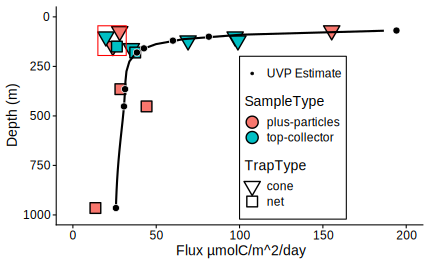
\includegraphics{../figures/FittedFlux.svg}

Figure 3. Particle flux, measured from sinking traps large symbols. Data
from the ``plus particles'' and ``top collector'' samples from both cone
and net traps were collated to generate these data. Trap types are shown
by the shape and color of the large points. Superimposed are binned
estemates of particle flux generated by fitting the sum of particle
numbers all four profiles, binned as in Figure X, to the trap observed
flux. The four points enclosed by the rectangle are unusually low
compared to other traps collected at the same depth, and were therefore
excluded from the fit. \{Convert UVP points to a line, maybe leave
points where the traps ares\}

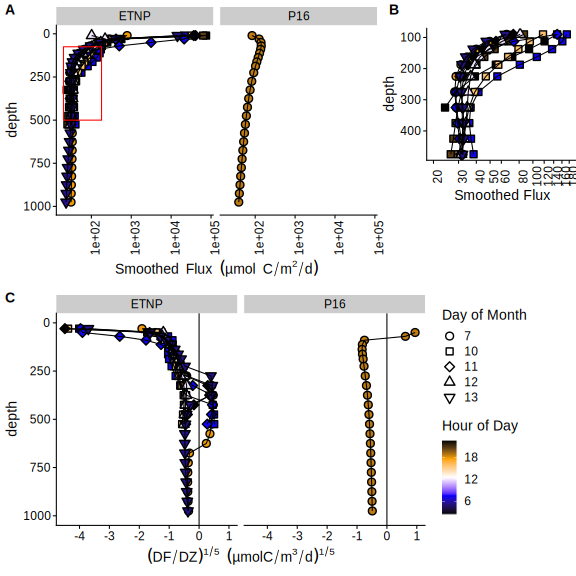
\includegraphics{../figures/FluxDeepDive.png}

Figure 4. Within and between day variability in UVP predicted particle
flux at ETNP station P2. Profiles are compared against P16 station 100,
a non OMZ station at similar latitude in the tropical pacific. All
profiles are depth binned with higher resolution towards the surface
(methods). \textbf{(A)} Flux profiles in the top 1000m of the water
column. \textbf{(B)} A more detailed depiction of the area enclosed by
the rectangle in \textbf{A}. \textbf{(C)} The rate of change of flux,
devided by the rate in change in depth. We show the fifth root of these
values in order to highlight differences between values close to zero.

\includegraphics{../figures/WBModelValidation.png}

Figure 5. \textbf{(A)} Gam smoothed binsize and volume particle numbers
at each particle size class. \textbf{(B)} Particle size distributions.
And estimated biomass of \textbf{(C)} Small and \textbf{(D)} Large
particles. \{I need to get rid of the green and blue line at P16 -- and
maybe calculate the photic zone therein\}.

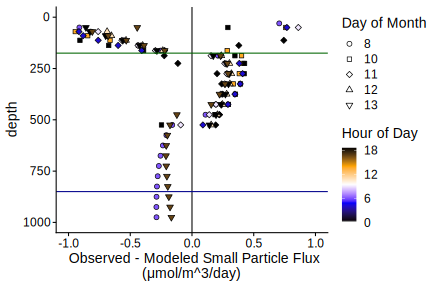
\includegraphics{../figures/FluxSizeShift.svg} Figure 9. Quantification
of non remineralization and sinking like processes. Points indicate the
difference between the observed small particle flux, and the flux that
would be estimated if particles from the size distribution in the depth
bin above remineralized and sank only following the PRiSM model. Values
are normalized to the change in depth. Thus values are uMol
Carbon/m3/day \{change to ``Deviation from Model'', keep units\}

\hypertarget{supplemental-figs}{%
\section{Supplemental Figs}\label{supplemental-figs}}

{[}move to supplement{]}

\includegraphics{../figures/stationP2_EK60_go7.png}

Figure S1. Acoustic data, measured by EK60, measured over the course of
the experiment. Shown are data from the all frequency bands. Values are
in return signal intensity and have not been normalized to observed
biomass.

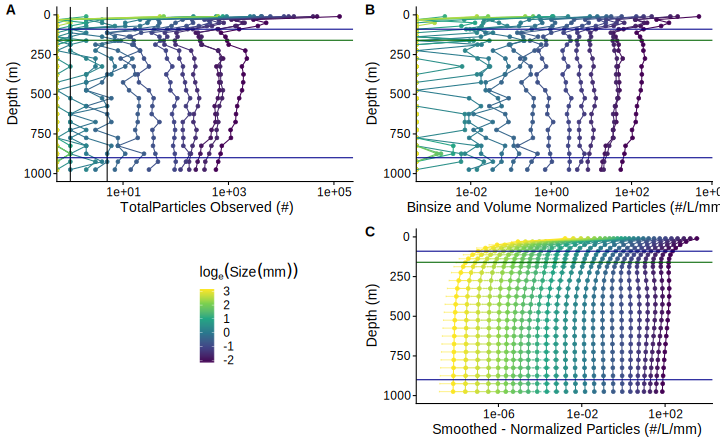
\includegraphics{../figures/AllParticleSizes.svg}

Figure S2. A profile of particle abundances at different sizes and
depths. \textbf{(A)} Numbers of observed particles and \textbf{(B)}
particle numbers normalized to volume sampled and particle size bin
width. \textbf{(C)} Smoothed and extrapolated particle abundances, based
on a negative bionomial gam that predicts particle abundance form size
and depth.

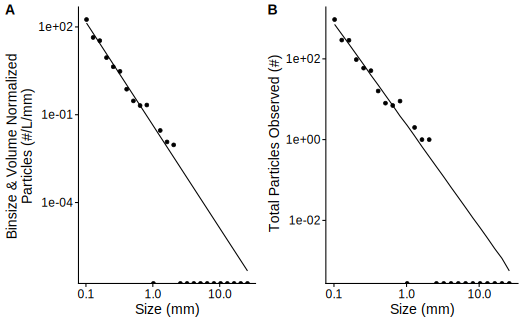
\includegraphics{../figures/ExamplePSD163m.svg}

Figure S2. An example of observed particle size distribution spectra.
These are depth binned data from between X and X m deep in the water
column from the cast that occurred at \emph{DATETIME for stn\_043}. A
total volume of XXX L of water are sampled herein. Points indicate
\textbf{(A)} total numbers of observed particles and \textbf{(B)}
particle numbers normalized to volume sampled and particle size bin
width. The line indicates the predicted best fit line of the data. The
line was fit on the bin and volume normalized data by a
negative-binomial general linear model. The line in panel \textbf{A}
indicates predictions from this same model, rescaled into absolute
particle space.

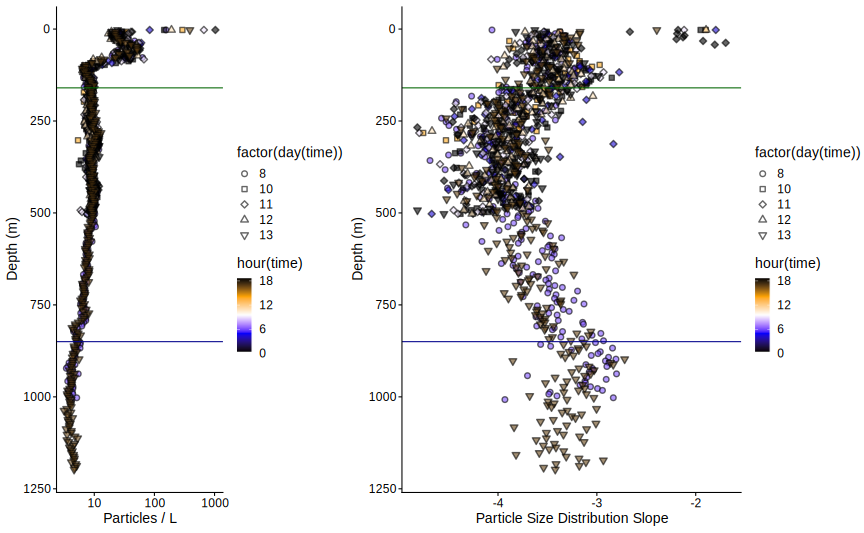
\includegraphics{../figures/ParticlesPSDMany.svg} Figure S3. (A)
Observed, volume normalized total particle numbers from 9 casts taken at
different times of the day at ETNP station P2. (B) Calculated particle
size distribution slopes of those particles. These data have not been
binnedby depth.

\includegraphics{../figures/CombinedP16S100Info.png}

Figure S4. Physical and chemical data from P16 Station 100. Located at
16.5°N 152.0°W. (A) Map of the nearby tropical pacific station P6
Station 100. Colors indicate chlorophyll concentrations at the surface,
averaged over all MODIS images. The red circle indicates the location of
Station P2. (B-D) Oceanographic parameters. The thin horizontal green
line shows the location of the base of the photic zone (200m m).
\textbf{A} Oxygen, and fluorescence. Because the fluorometer was broken
on this cruise, fluorescence data were pulled from world ocean atlas.
\textbf{B} Oxygen temperature and salinity. \textbf{(C)} Beam
attenuation and density, calculated from the salininity temperature and
pressure data.

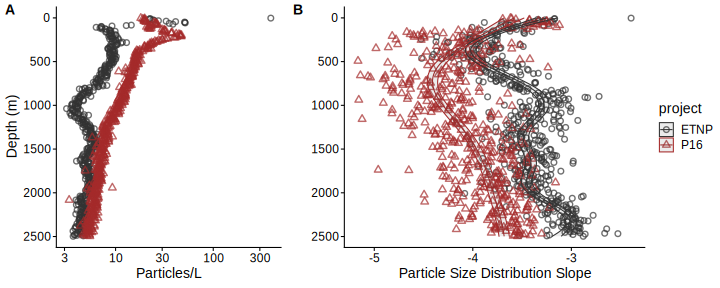
\includegraphics{../figures/ParticlesAndPSD_ETNPVsP16.svg} Figure S5. As
above, but for the final cast taken at ETNP station P2 and the only cast
collected from the P16 transect at the station 100. P16 Station 100 was
chosen because it is at a similar latitude to ETNP station P2. (A) Total
particle numbers, (B) Particle size distribution. \textbf{\{Cut to
1000m\}}

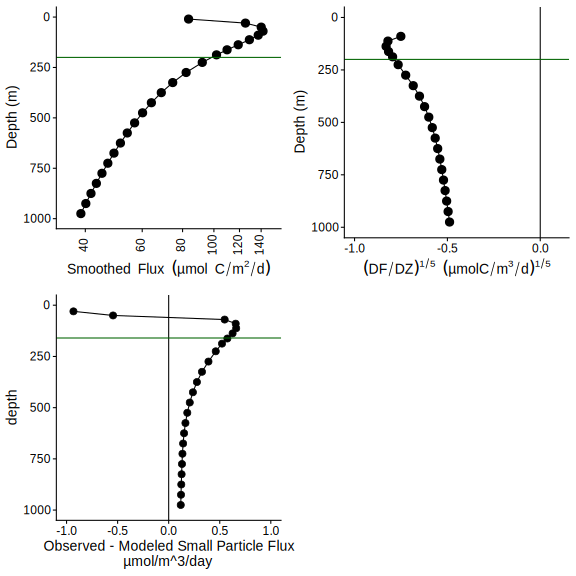
\includegraphics{../figures/P16FluxRelate.svg} Figure S6. Flux profiles
and flux attenuation at P2 Station 100. \textbf{(A)} Flux profile
\textbf{(B)} Fifth-root transformed depth normalized rate of flux
decrease. \textbf{(C)} Difference between observed and modeled results.
Higher values suggest more disaggregation-like processes.

\includegraphics{../figures/FluxGamPlot.png} Figure S\_. Gam predicted
effects of \textbf{A} Depth, \textbf{B} Day of the month in January
2017, and \textbf{C} hour of the day on the fifth-root transformed,
depth normalized, rate of change of flux. Y axis indicates the value of
the component smooth functions effect on Flux. Positive values associate
with times and regions of the water column where flux is increasing,
holding other factors constant, and negative ones where it is
decreasing.

\includegraphics{../figures/OSMSGamPlot.png}

Figure S\_. Gam predicted effects of \textbf{A} Depth, \textbf{B} Day of
the month in January 2017 Y axis indicates the value of the component
smooth functions effect on the difference between observed and modeled
flux. Thus higher values correspond with greater flux of small particles
than predicted by the model.

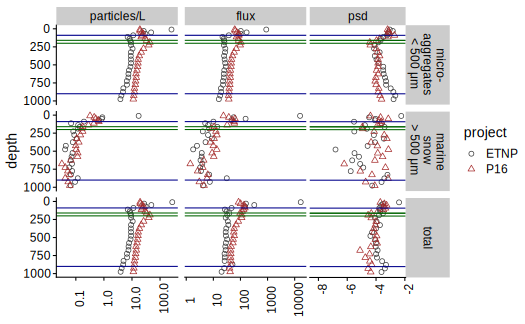
\includegraphics{../figures/BigVsSmall.svg} Figure S6. Depth binned
particle number (volume normalized), particle size slope (psd), and flux
(estimated as in Fig. 4) for large (\(>= 500\, \mu m\)), small
(\(< 500 \, \mu m\)) and total particles, at the oxic and anoxic site

\#MOVED Maybe skip? \{done, notadded\} Figure S1. A profile of data
generated by the UVP. At each depth the abundance of particles at each
size are color coded on a log scale. Particle sizes where no particles
in that sample were seen are represented with a smaller black dot.

\{done not added\} Figure S2. Comparason of total particle number and
particle size distributions of all casts taken at the ETNP station P2.
Points indicate individual samples, while ribbons indicate confedence
intervals of those sampeles. The overlapping confedence intervals
suggest that there is not a statistically detectable difference between
the different casts at the same station. \{I'd like a more quantitative
metric\}.

\hypertarget{references}{%
\section*{References}\label{references}}
\addcontentsline{toc}{section}{References}

\hypertarget{refs}{}
\leavevmode\hypertarget{ref-cavanRoleZooplanktonDetermining2017}{}%
Cavan, Emma L., Stephanie A. Henson, Anna Belcher, and Richard Sanders.
2017. ``Role of Zooplankton in Determining the Efficiency of the
Biological Carbon Pump.'' \emph{Biogeosciences} 14 (January): 177--86.
\url{https://doi.org/10.5194/bg-14-177-2017}.

\leavevmode\hypertarget{ref-cramRoleParticleSize2018}{}%
Cram, Jacob A., Thomas Weber, Shirley W. Leung, Andrew M. P. McDonnell,
Jun-Hong Liang, and Curtis Deutsch. 2018. ``The Role of Particle Size,
Ballast, Temperature, and Oxygen in the Sinking Flux to the Deep Sea.''
\emph{Global Biogeochemical Cycles} 32 (5): 858--76.
\url{https://doi.org/10.1029/2017GB005710}.

\leavevmode\hypertarget{ref-devriesMechanisticParticleFlux2014}{}%
DeVries, T., J.-H. Liang, and C. Deutsch. 2014. ``A Mechanistic Particle
Flux Model Applied to the Oceanic Phosphorus Cycle.''
\emph{Biogeosciences Discuss.} 11 (3): 3653--99.
\url{https://doi.org/10.5194/bgd-11-3653-2014}.

\leavevmode\hypertarget{ref-francoisFactorsControllingFlux2002}{}%
Francois, Roger, Susumu Honjo, Richard Krishfield, and Steve Manganini.
2002. ``Factors Controlling the Flux of Organic Carbon to the
Bathypelagic Zone of the Ocean.'' \emph{Global Biogeochemical Cycles} 16
(4): 34--31--34--20. \url{https://doi.org/10.1029/2001GB001722}.

\leavevmode\hypertarget{ref-gillyOceanographicBiologicalEffects2013}{}%
Gilly, William F., J. Michael Beman, Steven Y. Litvin, and Bruce H.
Robison. 2013. ``Oceanographic and Biological Effects of Shoaling of the
Oxygen Minimum Zone.'' \emph{Annual Review of Marine Science} 5 (1):
393--420. \url{https://doi.org/10.1146/annurev-marine-120710-100849}.

\leavevmode\hypertarget{ref-goldthwaitEffectsPhysicalFragmentation2005}{}%
Goldthwait, S. A., C. A. Carlson, G. K. Henderson, and A. L. Alldredge.
2005. ``Effects of Physical Fragmentation on Remineralization of Marine
Snow.'' \emph{Marine Ecology Progress Series} 305. Inter-Research
Science Center: 59--65.

\leavevmode\hypertarget{ref-goldthwaitQuantificationMarineSnow2004}{}%
Goldthwait, Sarah, Jeannette Yen, Jason Brown, and Alice Alldredge.
2004. ``Quantification of Marine Snow Fragmentation by Swimming
Euphausiids.'' \emph{Limnology and Oceanography} 49 (4): 940--52.
\url{https://doi.org/10.4319/lo.2004.49.4.0940}.

\leavevmode\hypertarget{ref-guidiRelationshipParticleSize2008}{}%
Guidi, Lionel, George A. Jackson, Lars Stemmann, Juan Carlos Miquel,
Marc Picheral, and Gabriel Gorsky. 2008. ``Relationship Between Particle
Size Distribution and Flux in the Mesopelagic Zone.'' \emph{Deep Sea
Research Part I: Oceanographic Research Papers} 55 (10): 1364--74.
\url{https://doi.org/10.1016/j.dsr.2008.05.014}.

\leavevmode\hypertarget{ref-kikoZooplanktonMediatedFluxesEastern2020}{}%
Kiko, Rainer, Peter Brandt, Svenja Christiansen, Jannik Faustmann, Iris
Kriest, Elizandro Rodrigues, Florian Schütte, and Helena Hauss. 2020.
``Zooplankton-Mediated Fluxes in the Eastern Tropical North Atlantic.''
\emph{Frontiers in Marine Science} 7 (May).
\url{https://doi.org/10.3389/fmars.2020.00358}.

\leavevmode\hypertarget{ref-kwonImpactRemineralizationDepth2009}{}%
Kwon, Eun Young, François Primeau, and Jorge L. Sarmiento. 2009. ``The
Impact of Remineralization Depth on the AirSea Carbon Balance.''
\emph{Nature Geoscience} 2 (9): 630--35.
\url{https://doi.org/10.1038/ngeo612}.

\leavevmode\hypertarget{ref-neuerOceanBiologicalCarbon2014}{}%
Neuer, Susanne, Morten Iversen, and Gerhard Fischer. 2014. ``The Ocean's
Biological Carbon Pump as Part of the Global Carbon Cycle.''
\emph{Limnology and Oceanography E-Lectures} 4 (4): 1--51.
\url{https://doi.org/10.4319/lol.2014.sneuer.miversen.gfischer.9}.

\leavevmode\hypertarget{ref-picheralUnderwaterVisionProfiler2010}{}%
Picheral, Marc, Lionel Guidi, Lars Stemmann, David M. Karl, Ghizlaine
Iddaoud, and Gabriel Gorsky. 2010. ``The Underwater Vision Profiler 5:
An Advanced Instrument for High Spatial Resolution Studies of Particle
Size Spectra and Zooplankton.'' \emph{Limnology and Oceanography:
Methods} 8 (9): 462--73. \url{https://doi.org/10.4319/lom.2010.8.462}.

\leavevmode\hypertarget{ref-steinbergZooplanktonOceanCarbon2017}{}%
Steinberg, Deborah K., and Michael R. Landry. 2017. ``Zooplankton and
the Ocean Carbon Cycle.'' \emph{Annual Review of Marine Science} 9:
413--44. \url{https://doi.org/10.1146/annurev-marine-010814-015924}.

\leavevmode\hypertarget{ref-steinbergBacterialVsZooplankton2008}{}%
Steinberg, Deborah K., Benjamin A. S. Van Mooy, Ken O. Buesseler, Philip
W. Boyd, Toru Kobari, and David M. Karl. 2008. ``Bacterial Vs.
Zooplankton Control of Sinking Particle Flux in the Ocean's Twilight
Zone.'' \emph{Limnology and Oceanography} 53 (4): 1327--38.
\url{https://doi.org/10.2307/40058255}.

\leavevmode\hypertarget{ref-strammaExpandingOxygenMinimumZones2008}{}%
Stramma, Lothar, Gregory C. Johnson, Janet Sprintall, and Volker
Mohrholz. 2008. ``Expanding Oxygen-Minimum Zones in the Tropical
Oceans.'' \emph{Science} 320 (5876): 655--58.
\url{https://doi.org/10.1126/science.1153847}.

\leavevmode\hypertarget{ref-turnerZooplanktonFecalPellets2015}{}%
Turner, Jefferson T. 2015. ``Zooplankton Fecal Pellets, Marine Snow,
Phytodetritus and the Ocean's Biological Pump.'' \emph{Progress in
Oceanography} 130 (January): 205--48.
\url{https://doi.org/10.1016/j.pocean.2014.08.005}.

\end{document}
